\documentclass[a4paper]{article}

% {{{ thai language support
% http://thaitug.daytag.org/wordpress/?p=1947
\usepackage{fontspec}
\usepackage{polyglossia}
\usepackage[Latin,Thai]{ucharclasses}
\defaultfontfeatures{Mapping=tex-text} 
\setdefaultlanguage{thai}
\setotherlanguage{english}
\newfontfamily{\thaifont}[Scale=MatchUppercase,Mapping=tex-text]{Norasi:script=thai}
\setTransitionTo{Thai}{\thaifont}
\setTransitionFrom{Thai}{\normalfont}
\XeTeXlinebreaklocale “th_TH” 
\XeTeXlinebreakskip = 0pt plus 1pt
\linespread{1.5}
% }}} end: thai language support

% remove visible box around the external URL
\usepackage[hidelinks]{hyperref}

% use fancybox to create the "Do you know?" box
\usepackage{fancybox}

% file path formatting
\usepackage{url}
\renewcommand\UrlFont{\thaifont\itshape}

% {{{ source code formatting
\usepackage{listings}
\usepackage{color}
\definecolor{dkgreen}{rgb}{0,0.6,0}
\definecolor{gray}{rgb}{0.5,0.5,0.5}
\definecolor{mauve}{rgb}{0.58,0,0.82}
\lstset{frame=tb, language=Java, aboveskip=3mm, belowskip=3mm,
  showstringspaces=false, columns=flexible, basicstyle={\small},
  numbers=none, numberstyle=\tiny\color{gray},
  keywordstyle=\color{blue}, commentstyle=\color{dkgreen},
  stringstyle=\color{mauve}, breaklines=true, breakatwhitespace=true,
  tabsize=3}
\lstset{numbers=left,numberstyle=\tiny,numbersep=5pt,language=Lisp,
  stringstyle=\small,basicstyle=\footnotesize,
  showstringspaces=false,breaklines}
% }}} end: source code formatting

% add ability to include pictures into the book
\usepackage{xcolor,graphicx}

% my package
\usepackage{p4bwcl}

\begin{document}

\title{Programming For Beginners With Common~Lisp}
\author{unsigned\_nerd}
\maketitle

\tableofcontents

\section{จุดเด่นของ Common Lisp คือความกระชับ}

การเขียนโปรแกรม คือ การเขียนชุดคำสั่งเพื่อสั่งให้คอมพิวเตอร์ทำงานตามที่เรากำหนด

เราเขียนชุดคำสั่งด้วย Programming Language

โดยทั่วไปหากเราพูดถึง Programming Language เราจะหมายถึงภาษาแบบ High-Level เช่น
Common Lisp, Python, Go, Java, PHP, Perl, C, JavaScript เป็นต้น
แต่ไม่ได้หมายถึงภาษา Assembly\footnote{ภาษา Assembly เป็น Low-Level
Programming Language}

แต่ละภาษาฯมีจุดเด่นที่แตกต่างกัน

ภาษา Common Lisp เป็นภาษาที่ปัจจุบันไม่ได้รับความนิยมเลยทั้งๆที่มี Feature ที่น่าสนใจต่างๆ%
มากมาย โดยเฉพาะอย่างยิ่ง Macro ใน Common Lisp ที่ทำให้เราสามารถเพิ่ม Syntax ต่างๆที่%
ต้องการเองได้ ทำให้เราสามารถเขียนโค้ดที่มีความกระชับและสั้นได้ง่าย\footnote{การเขียน%
โค้ดหากเขียนได้ยิ่งสั้นก็ถือว่ายิ่งดี โค้ดที่สั้นย่อมมีโอกาสเกิด Bug ได้น้อยกว่าโค้ดที่ยาว
อีกทั้งยังสามารถอ่านให้เข้าใจได้ง่ายกว่าอีกด้วย ท่านคงเคยได้ยินคำกล่าวที่ว่า การเขียน
Function ใดๆ ไม่ควรเขียนให้มีความยาวเกินความสูงของหน้าจอคอมฯของท่าน เพราะเมื่อมัน%
ยาวเกินไป สมองคนเราจะจำไม่ไหว} ตัวอย่างเช่น หากเราต้องการเขียนโปรแกรมที่ทำการ%
อ่านข้อมูลแบบ Plain Text จาก Standard Input
แล้วทำการใส่ Prefix String ``Common Lisp is fun?: " นำหน้าทุกบรรทัด
ก่อนที่จะพิมพ์ข้อมูลในแต่ละบรรทัดออกไปยัง Standard Output โดยปกติเราอาจเขียนโค้ดได้ดังนี้:

\begin{lstlisting}[caption=โค้ดแบบปกติ\label{lst:regular-print-each-line-code}]
(let (line)
  (loop for line = (read-line *standard-input* nil 'eof)
    until (eq line 'eof)
    do
      (format t ``Common Lisp is fun?  ~A~%" line)))
\end{lstlisting}

จะเห็นได้ว่ามันดูเข้าใจยากและมีรายละเอียดมาก ทั้ง loop, until, do, 'eof และ
nil แต่หากสมมุติว่าเราเขียน Macro ใน Common Lisp เป็น แล้วเราเขียน Macro ดังนี้:

\begin{lstlisting}[caption=Macro for-each-\$line-in \&
print-line\label{lst:macro-for-each-line-in-and-print-line}]
(defmacro for-each-$line-in (in-stream &rest body
  (let (($line (intern (symbol-name '$line))))
    `(let (,$line)
       (loop for ,$line = (read-line ,in-stream nil 'eof)
         until (eq ,$line 'eof)
         do
           ,@body))))

(defmacro print-line (formatted-string &rest args)
  `(format t ,(concatenate 'string formatted-string ``~%") ,@args))
\end{lstlisting}

จะทำให้เราสามารถเขียนโค้ดใหม่ได้ดังนี้:

\begin{lstlisting}[caption=โค้ดที่อ่านง่าย สบายตา ด้วยการใช้ Macro]
(for-each-$line-in *standard-input*
  (print-line ``Common Lisp is fun?  ~A" $line))
\end{lstlisting}

ซึ่งสั้นกว่าเดิมมาก และอ่านเข้าใจได้ง่าย

ท่านผู้อ่านที่ยังไม่ทราบว่า Macro คืออะไรอาจเห็นโค้ดนี้แล้วเข้าใจว่าสามารถใช้การเขียน
Function ทำได้เหมือนกัน ซึ่งหากลองดูดีๆจะพบว่าไม่สามารถทำได้ โดยมีจุดที่น่าสังเกตดังนี้

\begin{enumerate}
  \item มีการสร้างตัวแปรชื่อ \$line ขึ้นมาจาก Macro ชื่อ for-each-\$line-in โดยโค้ด%
    ที่เรียก Macro นี้สามารถนำตัวแปร \$line ไปใช้ต่อภายใน Loop ได้ด้วย
    เราไม่สามารถทำสิ่งนี้ได้ด้วย Function\footnote{เพราะ Function ใช้ Stack
    ทำให้พอ Function ทำการ Return แล้ว ตัวแปรต่างๆที่ได้ Define ไว้ใน Function
    นั้นๆก็จะถูกคืนหายไปหมด ในขณะที่ Macro จะทำงานตอน Compile Time} สิ่งนี้ศัพท์เทคนิค
    เรียกว่า Anaphoric Macro และ Intentional Variable
    Capture\footnote{\$line ที่อยู่ในชื่อ Function for-each-\$line-in เป็นเพียง%
    ส่วนหนึ่งของชื่อ Function เท่านั้น ผู้เขียนนิยมตั้งชื่อ Macro ที่เป็น Anaphoric
    Macro (คือ Macro ที่มีการ Define ตัวแปรออกมาให้ Caller ใช้) โดยการเขียนชื่อ%
    ตัวแปรที่ Macro สร้างขึ้นใส่ไว้ในชื่อ Function เลย (เช่นในกรณีนี้คือ \$line) จะได้%
    ดูได้ง่ายเวลาอ่านโค้ดว่าอะไรคือตัวแปรที่ Macro นั้นๆสร้างขึ้น}
  \item จะเห็นได้ว่า Definition ของ Macro for-each-\$line-in
    เป็นการลอกโค้ดแบบปกติใน Listing \ref{lst:regular-print-each-line-code} มาตรงๆ
    ซึ่งเป็นเรื่องที่ดีมาก เป็นการแสดงให้เห็นว่าการเขียน Macro เพื่อทำให้โค้ดกระชับแบบนี้เป็นเรื่องง่าย
    เมื่อเราเห็นโค้ดตรงไหนอ่านยาก ไม่อยากอ่าน เราก็ย้ายมันไปอยู่ใน Macro ได้ตรงๆเลย
    แต่ถ้าเราใช้ Function ทำแทนจะยุ่งยากกว่ามาก โดยเฉพาะการส่ง Source Code
    ผ่าน Parameter ชื่อ body จะไม่สามารถทำได้
  \item Definition ของ Macro ดูเข้าใจยากและซับซ้อน แต่นั่นไม่ใช่ปัญหา เป้าประสงค์%
    ของการใช้ Macro คือการ Encapsulate ความยุ่งยากให้อยู่ใน Macro แล้วทำให้โค้ดที่%
    เรียกใช้ (Caller) อ่านง่าย
\end{enumerate}

\section{ความไม่ดังของ Common Lisp}

สามารถดูการจัดอันดับภาษาคอมฯที่ได้รับความนิยมล่าสุดได้ที่นี่: \href{http://pypl.github.io/PYPL.html}{http://pypl.github.io/PYPL.html}

ณ วันที่ 30 พฤษภาคม 2563 อันดับหนึ่งคือภาษา Python ส่วนภาษา Common Lisp ไม่ติดอันดับบน PYPL เลย

ทาง PYPL แนะนำว่าถ้าหากอยากทราบความนิยมของภาษาที่ไม่ติดอันดับให้ใช้ Google Trends ดู

เมื่อลองใช้ Google Trends เปรียบเทียบความนิยมระหว่าง 3 ภาษา ได้แก่ Python, PHP
และ Common Lisp เราจะพบว่ากระแสความนิยมในภาษา Common Lisp นั้นต่ำมาก
ดังจะเห็นได้จากรูปที่ \ref{lang-pop}:

\begin{figure}[!hbtp]
  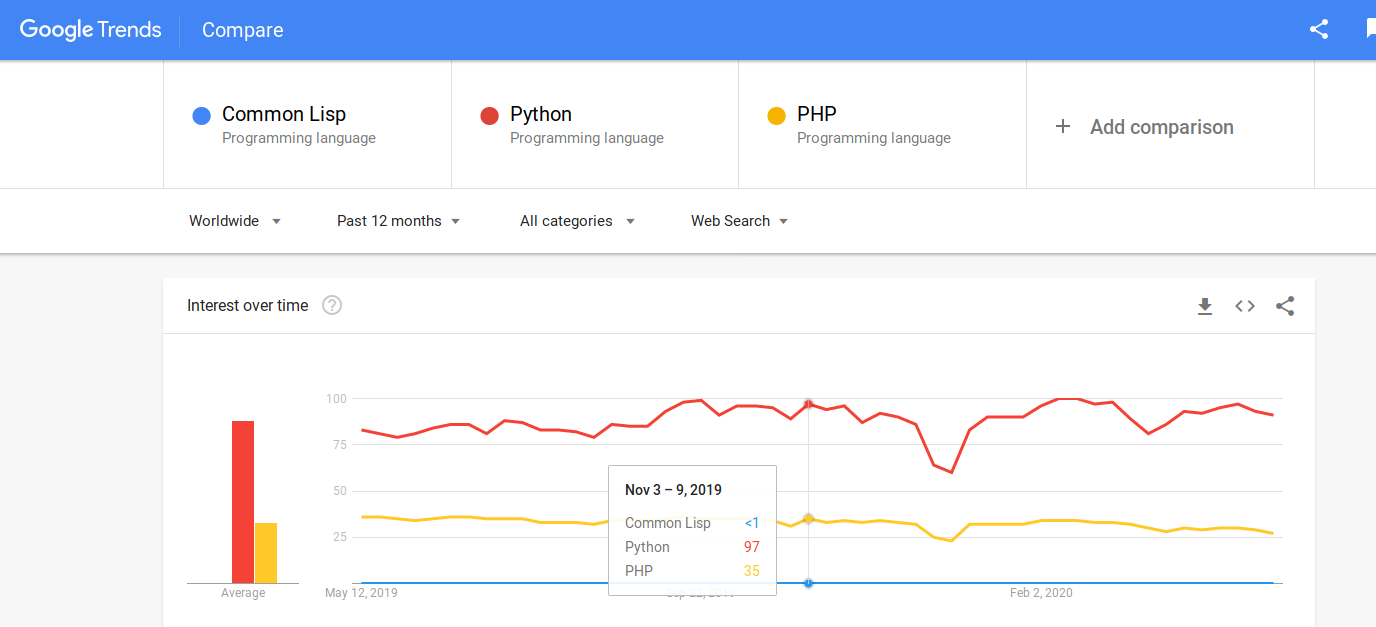
\includegraphics[width=\linewidth]{images/lang-popularity.png}
  \caption{Language popularity\label{lang-pop}}
\end{figure}

อย่างไรก็ตาม แม้ว่า Common Lisp จะไม่ได้รับความนิยมในปัจจุบัน
แต่ก็ไม่ได้หมายความว่ามันจะไม่เหมาะกับการใช้เป็นเครื่องมือในการเรียนรู้การเขียนโปรแกรม%
สำหรับมือใหม่

เมื่อท่านได้เรียนรู้การเขียนโปรแกรมด้วยภาษา Common Lisp แล้ว ท่านจะสามารถเรียนภาษา%
คอมฯอื่นๆเพิ่มเติมได้ง่ายขึ้นมาก

เป็นที่ยอมรับกันโดยทั่วไปว่าในชีวิตหนึ่งๆของคนเรา เราย่อมต้องเรียนภาษาคอมพิวเตอร์หลาย%
ภาษากันอยู่แล้ว แล้วทำไมจึงไม่ลองเรียนภาษา Common Lisp กันเล่า!

\doyouknow{
  ภาษา Logo (เจ้าเต่าน้อย Logo) ที่หลายๆท่านอาจได้เคยเรียนในสมัยเด็กๆเป็น
    Dialect หนึ่งของภาษา Lisp นี่ก็ยิ่งชี้ให้เห็นว่า Common Lisp
    เหมาะกับการเป็นภาษาเขียนโปรแกรมแรกๆของทุกท่านขนาดไหน
}

\section{Common Lisp Package, ASDF, System และ Quicklisp}

เรื่อง Package, ASDF, System และ Quicklisp
เป็นเรื่องหนึ่งที่ผู้เขียนมีความสับสนมากในช่วงเริ่มต้นของการเรียนภาษา Common Lisp

ความยืดหยุ่นที่มากเกินไป กับ Documentation ที่ไม่ดีนักก็ทำให้เกิดผลเสียต่อความนิยมของภาษา%
คอมฯหนึ่งๆได้

เรื่องนี้เกี่ยวกับระบบ Software Library ใน Common Lisp

สำหรับมือใหม่ ให้ลองทำตามนี้ก่อน จะได้ไม่สับสน แล้วเมื่อเชี่ยวชาญแล้วค่อยปรับแต่งตามใจชอบ

Software Library ต่างๆใน Common Lisp จะอยู่ในสิ่งที่เรียกว่า System

System หนึ่งๆจะประกอบไปด้วย Package ตั้งแต่ 1 อันขึ้นไป โดยจะใช้ ASDF เป็นเครื่องมือ%
ในการระบุว่าไฟล์ต่างๆของ Package ทั้งหลายน้้นอยู่ตรงไหน ในขณะที่ Quicklisp จะเป็น%
โปรแกรมที่ใช้ติดตั้ง 3rd Party System จาก Software Repository ของ
Quicklisp\footnote{ภายใน Quicklisp ก็ใช้ ASDF ในการจัดการ System เช่นกัน}
ยกตัวอย่างเช่น หากเราต้องการใช้ Regular Expression เราก็สามารถใช้ Quicklisp
ทำการดาวน์โหลดและติดตั้ง System ชื่อ cl-ppcre ได้

เวลาเราจะสร้าง Project ใหม่ สมมุติว่าชื่อ hello-world ให้เราไปที่ Directory ชื่อ
\path{~/common-lisp/} แล้วสร้าง directory ชื่อ \path{hello-world/} ขึ้นมา
ซึ่งจะเป็นที่ๆเราจะใส่ Source Code ของเราในนั้น\footnote{แนะนำให้เก็บ Project
ทั้งหมดภายใน Directory ชื่อ \path{~/common-lisp/} เพราะ Directory นี้เป็นหนึ่งในรายการ
Default Directory ที่ ASDF ใช้ในการหา System หากท่านผู้อ่านต้องการเก็บ Common
Lisp Project ของท่านไว้ใน Directory อื่น สามารถศึกษาวิธีการได้จากคู่มือของ ASDF}

\section{การติดตั้งระบบเพื่อเริ่มเขียนโปรแกรมด้วยภาษา Common Lisp}

Common Lisp มีหลาย Implementation เราเลือกใช้ Sbcl ซึ่งเป็น Common Lisp Implementation ที่ได้รับความนิยมที่สุด

ผู้เขียนใช้ Debian 10 เป็น Operating System

ทำการติดตั้ง Sbcl, Quicklisp และ un-utils บนคอมฯของท่านโดยทำตามขั้นตอนในลิงค์นี้:
\href{https://github.com/unsigned-nerd/un-utils}{https://github.com/unsigned-nerd/un-utils}

\subsection{Sbcl}

ดังได้กล่าวไปก่อนหน้านี้ Sbcl เป็น Implementation หนึ่งของ Common Lisp

เป็นโปรแกรมที่ใช้รันโปรแกรมที่เราเขียนขึ้นด้วยภาษา Common Lisp

\subsection{Quicklisp}

Quicklisp เป็นโปรแกรมเชิงระบบที่นิยมใช้ในการติดตั้ง System ต่างๆจากผู้พัฒนาคนอื่น

โดยทั่วไป ให้เราคิดเสียว่า หากเราต้องการดาวน์โหลด System ของคนอื่นมาใช้
โดยคิดว่าจะใช้อย่างเดียว ไม่ได้ต้องการจะแก้ไขอะไรมัน ก็ควรจะใช้ Quicklisp
ในการดาวน์โหลดและติดตั้ง

แต่ถ้าเราต้องการเขียน System เอง หรือ ต้องการแก้ไข System ของผู้อื่น ก็ให้ใช้เครื่องมือชื่อ
ASDF ในการจัดการ

ASDF เป็นเครื่องมือที่ใช้ในการจัดการ

\subsection{un-utils}

un-utils เป็น Common Lisp System ที่ทางผู้เขียนพัฒนาขึ้นมา ซึ่งมี Package ที่น่าสนใจชื่อ
un-utils.simple-syntax

Package นี้จะมี Macro ต่างๆที่ช่วยทำให้เขียนโค้ดได้ง่ายขึ้นสำหรับมือใหม่อย่างผู้เขียนที่ยังไม่ชิน%
กับ Default Macro ต่างๆของ Common Lisp

ผู้เขียนเห็นว่า Default Macro ของ Common Lisp ที่มักใช้บ่อยเช่น loop หรือ do อ่านยาก%
จึงทำการเขียน Macro ครอบมัน เพื่อให้ผู้เขียนสามารถเขียนโปรแกรมได้ง่ายขึ้น\footnote{%
และนี่ก็เป็นจุดแข็งหนึ่งของ Common Lisp นั่นเอง นั่นคือความสามารถในการปรับเปลี่ยน Syntax
ของภาษาให้ตรงตามความต้องการของเรา} ซึ่งก็คือ Macro อย่างที่ท่านได้เห็นตัวอย่างไปแล้วใน
Listing \ref{lst:macro-for-each-line-in-and-print-line} นั่นเอง

\end{document}

% todo
%
% - what other langs have
%   - list comprehension in python
%   - with statement
%
